% this metadata is for the tagging setup please see: https://latex3.github.io/tagging-project/documentation/usage-instructions
\DocumentMetadata{
  lang        = en,
  pdfstandard = ua-2,
  pdfstandard = a-4, 
  tagging=on,
  tagging-setup={math/setup=mathml-SE} 
}
\documentclass[12pt]{article}

\usepackage[letterpaper,top=2cm,bottom=2cm,left=3cm,right=3cm,marginparwidth=1.75cm]{geometry}
\usepackage{amsmath}
\usepackage{unicode-math}
\usepackage{graphicx}
\usepackage{parskip}
\usepackage{url}
\usepackage[hidelinks]{hyperref}
\usepackage{hyperref}
\hypersetup{
    pdftitle={Accessible LaTeX example}, % Satisfies the mandatory dc:title requirement
    pdfauthor={Overleaf Support},          % Optional, but good practice
    pdfdisplaydoctitle=true         % Crucial: instructs the PDF viewer to display the title instead of the filename
}

\title{Accessible LaTeX example}
\author{Overleaf Support}

\begin{document}
\maketitle

\begin{abstract}
A simple \LaTeX{} document authored using Overleaf. This document takes advantage of the PDF tagging support provided by the \LaTeX{} team that is available in TeXLive 2025.
\end{abstract}

\section{Introduction}

This simple example describes some of the considerations that go into creating accessible documents with \LaTeX{} using Overleaf.

\subsection{Selecting the TeX Live version in Overleaf}

Overleaf uses a standard TeX Live \LaTeX{} environment, making the accessibility support that is being provided by the \href{https://www.latex-project.org/}{\texorpdfstring{\LaTeX{}}{LaTeX} team} available to all Overleaf users.

With 2025 TeX Live, \LaTeX{} can now produce tagged PDFs automatically -- a key requirement for accessibility. Additional accessibility features are being added on an ongoing basis to the TeX Live builds. Currently, \href{https://www.overleaf.com/blog/tex-live-2025-is-now-available}{new projects created in Overleaf} use the 2025 TeX Live tested release, and for those who need even more recent releases, a rolling updated version of TeX Live is available through our \href{https://www.overleaf.com/labs/participate}{Overleaf Labs} program. For most requirements, the standard 2025 TeX Live image should be sufficient, but for those who wish to use the most recent features provided by the \LaTeX{} team, the rolling version provided by Overleaf Labs may be required.

\subsection[Including DocumentMetadata]{Including \texttt{DocumentMetadata}}

A key requirement for setting up the tagging support is to include the \texttt{DocumentMetadata} prior to the \verb|\documentclass| declaration. Please see the \LaTeX{} team's \href{https://latex3.github.io/tagging-project/documentation/usage-instructions}{tagging usage instructions} for details.

\begin{figure}
\begingroup
\begin{verbatim}
\DocumentMetadata{
  lang        = en,
  pdfstandard = ua-2,
  pdfstandard = a-4, 
  tagging=on,
  tagging-setup={math/setup=mathml-SE} 
}    
\end{verbatim}
\caption[The DocumentMetadata used in this document]{The \texttt{DocumentMetada} used in this document}
\endgroup
\end{figure}

\section{Tagging special structures}

The automatic tagging provided now in \LaTeX{} doesn't guarantee accessibility. Having an error-free document, that uses standard \LaTeX{} commands (for sections, lists, etc.) is also essential.

\subsection{Remember to include alternate text for images}

For figures, you can use the \texttt{alt} optional parameter to the \verb|\includegraphics| command that is provided with the \texttt{graphicx} package.


\begin{figure}[!htb]
\centering
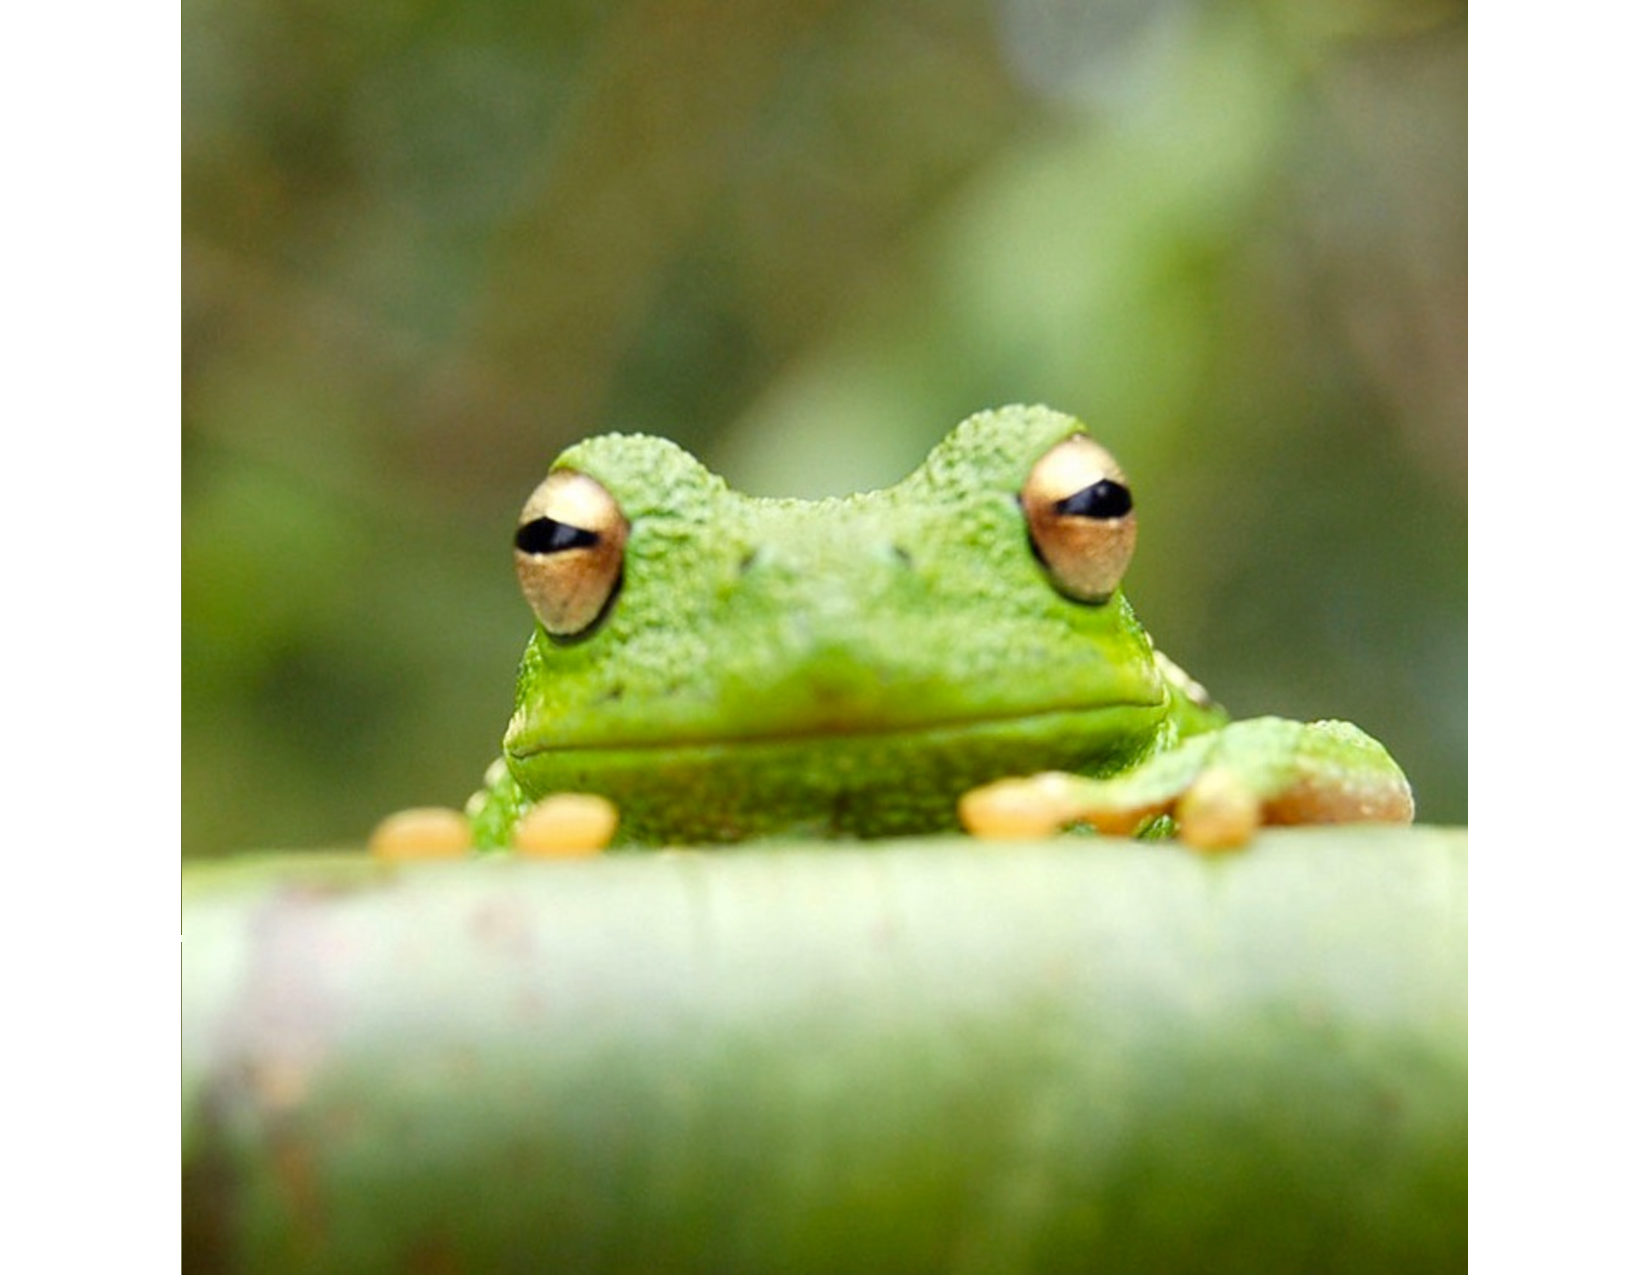
\includegraphics[width=0.25\linewidth,alt={image of a frog facing  towards the reader}]{frog.pdf}
\caption{This image has some alt text}
\label{fig:frog}
\end{figure}
\setkeys{Gin}{alt={}} % <--- This resets the alt text for all following images


\subsection{Tagging tables}

Use the table and tabular environments for basic tables --- see Table~\ref{tab:widgets}.

For tables, you should include the command that will identify the header row, which would typically be the first row: \verb|\tagpdfsetup{table/header-rows={1}}|.

\tagpdfsetup{table/header-rows={1}} %this tells the tagging infrastructure what row is the header of the table
\begin{table}[!htb]
\centering
\begin{tabular}{l|r}
Item & Quantity \\\hline
Widgets & 42 \\
Gadgets & 13
\end{tabular}
\caption{An example table.}
\label{tab:widgets}
\end{table}

\subsection{How to write accessible mathematics}

\LaTeX{} is great at typesetting mathematics. 

For equations, you should compile with \texttt{LuaLaTeX }if possible to generate the \texttt{MathML}. If you compile with \texttt{LuaLaTeX} and include the \verb|tagging-setup={math/setup=mathml-SE}| option, \texttt{MathML} versions of the equations will be added into the tagged PDF directly.

Below is some example mathematics, which will be properly tagged and provided with its \texttt{MathML} translation in the final PDF

Let $X_1, X_2, \ldots, X_n$ be a sequence of independent and identically distributed random variables with $\text{E}[X_i] = \mu$ and $\text{Var}[X_i] = \sigma^2 < \infty$, and let
\[S_n = \frac{X_1 + X_2 + \cdots + X_n}{n}
      = \frac{1}{n}\sum_{i}^{n} X_i\]
denote their mean. Then as $n$ approaches infinity, the random variables $\sqrt{n}(S_n - \mu)$ converge in distribution to a normal $\mathcal{N}(0, \sigma^2)$.

\section{Other accessibility considerations}

While PDF tagging is a key criteria that many accessibility verification systems check for, accessibility criteria and testing can vary, and the efficacy of tagged PDFs can vary with different assistive technologies. 

It is recommended that you validate sample tagged PDFs according to the criteria set by your institution, and test using the assistive technologies that have been adopted by your users.

\section{Other formats}
In addition to PDF output, it is also possible to compile to HTML using \texttt{latexml} and \texttt{bookml}.

When using Overleaf, the \href{https://docs.overleaf.com/integrations-and-add-ons/git-integration-and-github-synchronization/github-synchronization}{GitHub synchronization} feature makes it possible to run these tools outside of Overleaf as GitHub workflows.

\nocite{*}
\bibliographystyle{alpha}
\bibliography{references}

\end{document}
